
\subsubsection{Primary Finding: Alignment Signal Fails on Both Datasets}

\textbf{Table 1:} Gradient alignment vs. per-sample loss ROC-AUC at checkpoint epochs.

\begin{table*}[htbp]
\centering
\resizebox{\dimexpr 2\columnwidth+\columnsep\relax}{!}{%
\begin{tabular}{lllllll}
\toprule
Epoch & WB Align & WB Loss & WB Gap† & CelebA Align & CelebA Loss & CelebA Gap† \\
\midrule
1 & 0.150 & 0.930 & $-0.780$ & 0.246 & 0.975 & $-0.729$ \\
5 & 0.301 & 0.854 & $-0.554$ & 0.484 & 0.949 & $-0.465$ \\
10 & 0.340 & 0.821 & $-0.481$ & 0.523 & 0.939 & $-0.416$ \\
25 & 0.340 & 0.801 & $-0.503$ & 0.407 & 0.910 & $-0.503$ \\
50 & 0.349 & 0.775 & $-0.426$ & 0.632 & 0.905 & $-0.273$ \\
\bottomrule
\end{tabular}
}
\end{table*}

\textit{† Gap = Align $-$ Loss; negative values indicate alignment below loss. Values rounded to three decimal places from raw results (e.g., WB epoch 1: alignment = 0.1495, loss = 0.9297). See \texttt{h-e1/experiment\textbackslash \_results.json} for full precision.}

\begin{figure}[htbp]
\centering
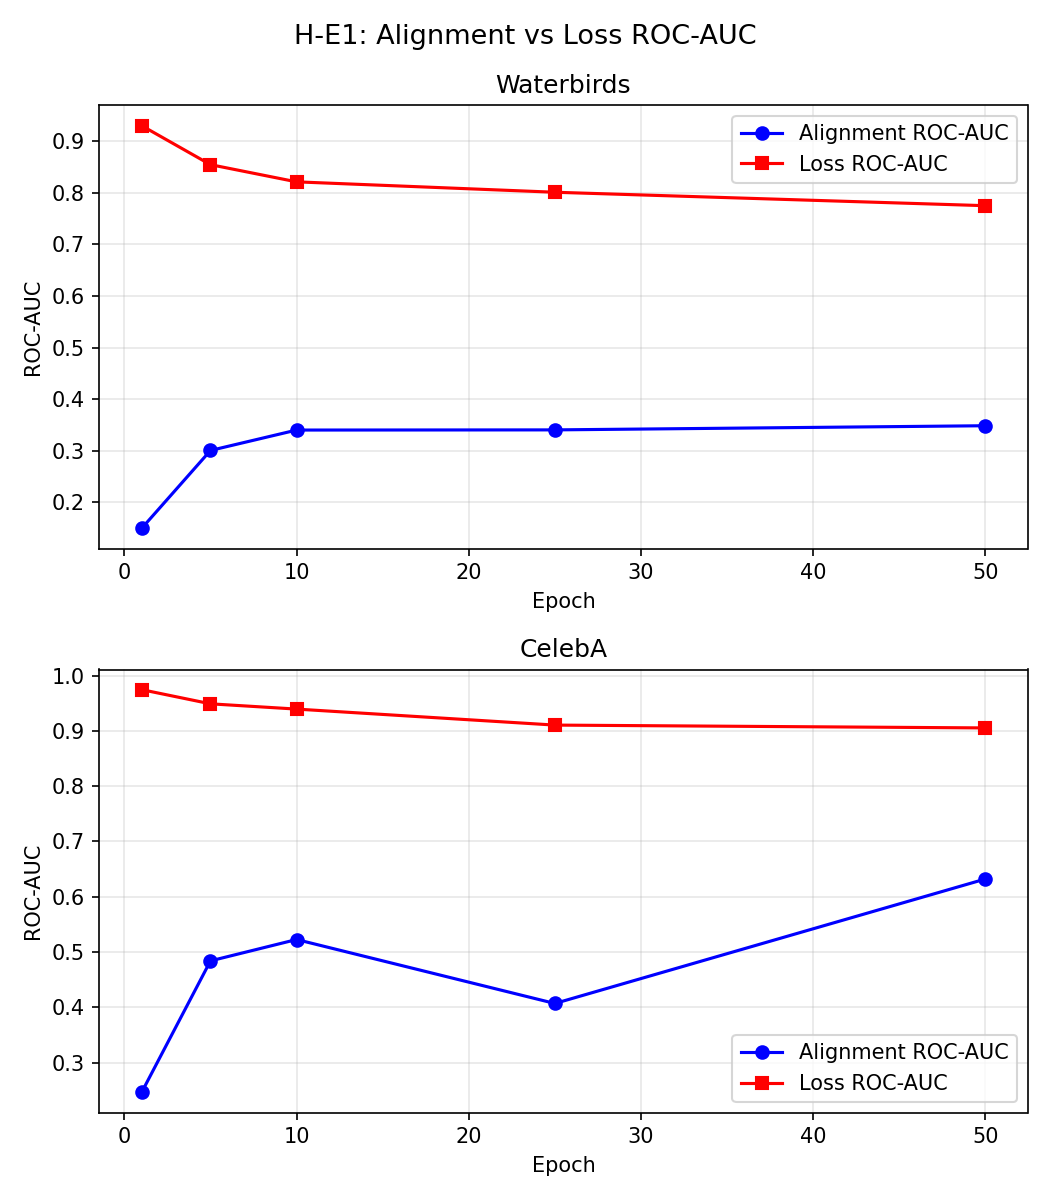
\includegraphics[width=\columnwidth]{figures/roc_auc_vs_epoch.png}
\caption{ROC-AUC vs. training epoch for gradient alignment score and per-sample loss, Waterbirds and CelebA combined}
\label{fig:roc_auc_vs_epoch}
\end{figure}

\textbf{Figure 1:} ROC-AUC vs. training epoch for gradient alignment score (lower curves) and per-sample loss (upper curves), on Waterbirds (solid lines) and CelebA (dashed lines). The alignment ROC-AUC remains far below loss ROC-AUC at all epochs on both datasets. The dotted horizontal line at 0.5 marks chance-level performance; alignment falls below chance on Waterbirds throughout training. Source: \texttt{h-e1/figures/roc\textbackslash \_auc\textbackslash \_vs\textbackslash \_epoch.png}.

\subsubsection{The Alignment Inversion Effect on Waterbirds}

At epoch 1 on Waterbirds: alignment ROC-AUC = \textbf{0.150} (raw value: 0.1495), substantially below chance (0.5). The conflict score $a_i$ (negated cosine similarity) is anti-predictive: minority samples score \textit{lower} on $a_i$ than majority samples, meaning minority samples have \textit{higher} raw cosine similarity with the within-batch mean --- the direct opposite of the hypothesis. The signal moves toward chance by epoch 50 (0.349) but alignment never approaches discriminative territory at any tested epoch. The gap to loss remains 0.43--0.78 throughout training.

\begin{figure}[htbp]
\centering
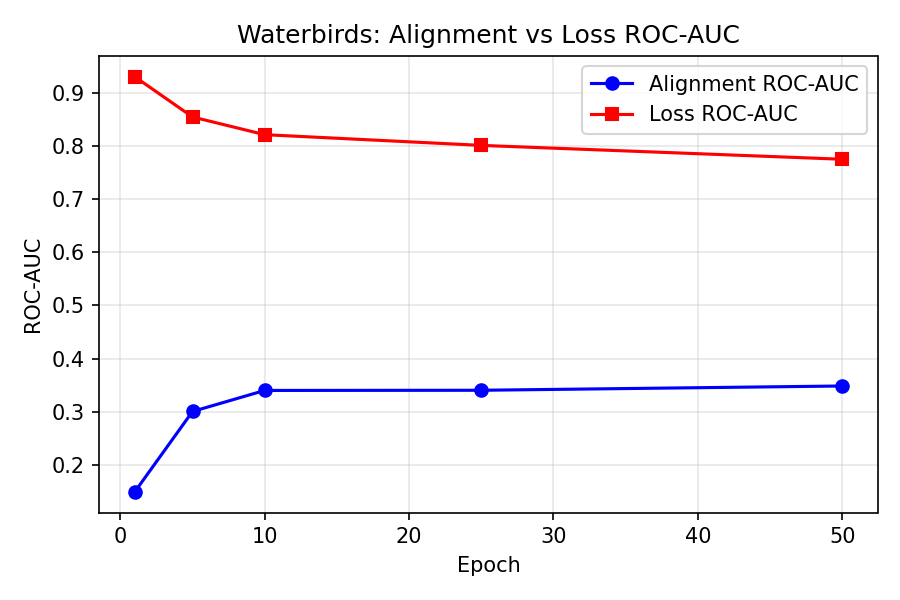
\includegraphics[width=\columnwidth]{figures/roc_auc_vs_epoch_waterbirds.png}
\caption{ROC-AUC vs. training epoch, Waterbirds only}
\label{fig:roc_auc_vs_epoch_waterbirds}
\end{figure}

\textbf{Figure 2:} Waterbirds detail. Alignment ROC-AUC (0.150--0.349) vs. loss ROC-AUC (0.775--0.930) across epochs 1--50. The alignment curve remains below the dashed chance line (0.5) at all tested epochs; the loss curve begins near 0.93 and degrades monotonically as the model memorizes training samples. Source: \texttt{h-e1/figures/roc\textbackslash \_auc\textbackslash \_vs\textbackslash \_epoch\textbackslash \_waterbirds.png}.

\subsubsection{Temporal Dynamics on Waterbirds}

On Waterbirds, per-sample loss ROC-AUC begins high (0.930 at epoch 1) and monotonically degrades to 0.775 at epoch 50 as the model memorizes training samples (training loss = 0.174 at epoch 1, approaching near-zero at 0.0003 by epoch 50). Gradient alignment begins inverted and slowly improves --- converging toward loss from below, as near-zero training loss collapses all gradient discriminability.

\subsubsection{CelebA: Weak Positive Signal at Late Epochs}

CelebA alignment begins inverted (0.246 at epoch 1), recovers through epoch 10 (0.523), dips at epoch 25 (0.407), then peaks at epoch 50 (0.632). It remains 0.273 below loss (0.905) at best. The weaker inversion is consistent with batch contamination being prevalence-dependent: at ~0.8\% minority prevalence and B=32, the expected number of minority samples per batch is approximately 0.26, substantially reducing their contamination impact on the within-batch mean compared to Waterbirds (~5\% minority, 1--2 samples per batch).

\begin{figure}[htbp]
\centering
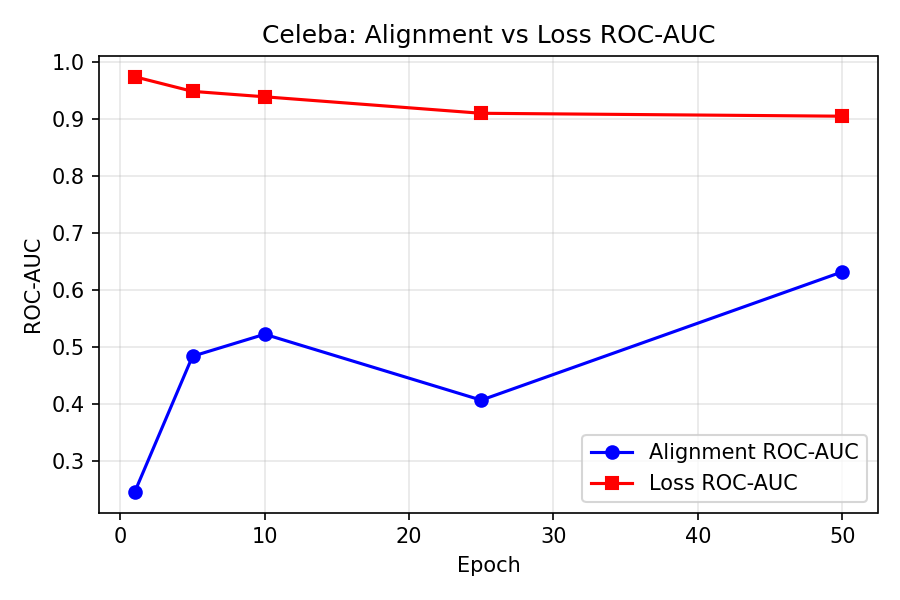
\includegraphics[width=\columnwidth]{figures/roc_auc_vs_epoch_celeba.png}
\caption{ROC-AUC vs. training epoch, CelebA only}
\label{fig:roc_auc_vs_epoch_celeba}
\end{figure}

\textbf{Figure 3:} CelebA detail. Alignment ROC-AUC (0.246--0.632) vs. loss ROC-AUC (0.905--0.975) across epochs 1--50. Alignment shows a non-monotonic trajectory, dipping at epoch 25 before recovering to 0.632 at epoch 50. The gap at the best alignment epoch (epoch 50) is 0.273. Source: \texttt{h-e1/figures/roc\textbackslash \_auc\textbackslash \_vs\textbackslash \_epoch\textbackslash \_celeba.png}.

Score distributions and full ROC curves are presented in the Appendix (Figures 4--7).

